\section{Butterfly board}

\subsection{Making connections}
Figure \ref{fig:bfly_connect} shows the connections that should be made to
the Butterfly board.

\begin{figure}[ht]
  \begin{center}
    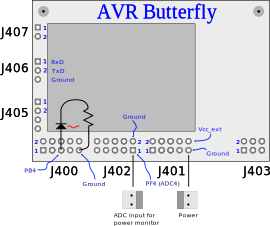
\includegraphics[clip,scale=1]{figs/butterfly_connect}
    \caption{Connections to the AVR Butterfly \label{fig:bfly_connect}}
  \end{center}
\end{figure}

Figure \ref{fig:uart_cable} shows how the UART cable should be made.
\begin{figure}[ht]
  \begin{center}
    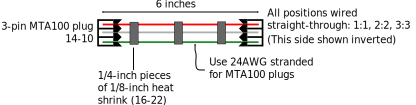
\includegraphics[clip,scale=1]{figs/uart_cable}
    \caption{The UART cable connecting the Butterfly and USB
      boards.\label{fig:uart_cable}}
  \end{center}
\end{figure}

Figure \ref{fig:bfly_power_cable} shows how to make the power cable.
\begin{figure}[ht]
  \begin{center}
    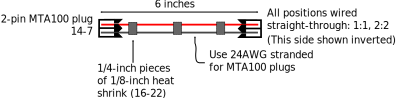
\includegraphics[clip,scale=1]{figs/butterfly_power_cable}
    \caption{The power cable connecting the Butterfly and the USB
      boards.  The cable should run from J400 on the USB board to the
      power connector shown in figure
      \ref{fig:bfly_connect}.\label{fig:bfly_power_cable} }
  \end{center}
\end{figure}

Figure \ref{fig:isense_cable} shows how to make the cable connecting
the USB board's current sense output to the Butterfly's ADC input.
\begin{figure}[ht]
  \begin{center}
    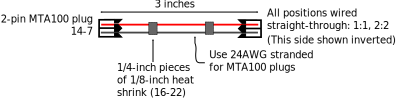
\includegraphics[clip,scale=1]{figs/current_sense_cable}
    \caption{The cable connecting the Butterfly board's power monitor
      input to the USB board's output.\label{fig:isense_cable} }
  \end{center}
\end{figure}


